\chapter{Álgebra Abstrata}

A álgebra abstrata é o ramo da matemática que estuda estruturas algébricas,
como grupos, anéis e corpos, focando nas propriedades de operações
independentemente dos objetos específicos sobre os quais elas atuam. Essas
estruturas fornecem uma linguagem unificada para generalizar e abstrair
operações algébricas, permitindo a resolução de problemas complexos em diversas
áreas da matemática e suas aplicações.

A álgebra abstrata é fundamental tanto na matemática pura quanto em aplicações
práticas. Na teoria dos números, ela sustenta o estudo de equações diofantinas
e criptografia moderna. Na geometria, fornece ferramentas para analisar
simetrias. Na ciência da computação e na teoria da codificação, corpos finitos
e espaços vetoriais são essenciais para desenvolver códigos de correção de
erros e algoritmos eficientes.

Neste capítulo, iremos realizar um digressão sobre este tema, introduzindo os
conceitos algébricos necessários para o estudo da teoria da codificação.


\section{Contexto Histórico do Desenvolvimento da Álgebra Abstrata}

O desenvolvimento da álgebra abstrata foi um processo gradual e complexo.
Inicialmente focada em polinômios e equações (com raízes na antiguidade e
avanços no Renascimento), a álgebra passou por uma transformação no século XIX.
Essa transformação envolveu uma mudança de foco: a álgebra tradicional,
centrada na resolução de equações, evoluiu para a álgebra abstrata, que surge
como uma forma de generalização e unificação de diversas abordagens e
ferramentas matemáticas, estudando estruturas algébricas gerais e suas
propriedades. Problemas como a não resolubilidade de equações de grau 5 ou
maior \parencite{abel1826memoire} e a teoria de \textcite{galois1832memoire} sobre simetrias de raízes de polinômios
impulsionaram essa mudança, introduzindo o conceito de grupo. Contribuições da
teoria dos números \parencite{gauss1801disquisitiones}, geometria \parencite{klein1926vorlesungen} e análise também foram cruciais.
No início do século XX, a álgebra abstrata se consolidou com a formalização de
estruturas como grupos, anéis e corpos \parencite{noether1921idealtheorie,van1930moderne,artin1991algebra},
unificando diversas áreas da matemática. É importante notar que esse
desenvolvimento histórico é bem diferente da forma como as ideias são
frequentemente apresentadas em livros didáticos, onde a apresentação é formal e
segue um desenvolvimento sequencial, contrastando com a natureza complexa e
ramificada do processo histórico real, que envolveu um longo período de
unificação e estruturação.

%O desenvolvimento da álgebra abstrata é uma história de unificação gradual,
%marcada por um caminho longo, tortuoso e repleto de debates. Antes do século
%XIX, a álgebra era essencialmente o estudo de polinômios e suas equações, com
%métodos voltados para resolver problemas específicos em aritmética e geometria.
%Suas raízes remontam à antiguidade, com babilônios e egípcios resolvendo
%equações lineares e quadráticas de forma prática, mas sem uma teoria geral. No
%Renascimento, matemáticos como Cardano e Tartaglia avançaram na resolução de
%equações cúbicas e quárticas, mas ainda de maneira ad hoc, sem uma estrutura
%unificada.
%
%No século XVII, François Viète introduziu o simbolismo algébrico, permitindo
%expressar equações de forma geral, o que marcou o início de uma álgebra mais
%abstrata. Contudo, o impulso definitivo para a álgebra abstrata moderna veio no
%século XIX, motivado por problemas que desafiavam as ferramentas algébricas
%tradicionais. Um desses problemas foi a resolubilidade de equações polinomiais
%de grau superior. Niels Henrik Abel demonstrou que equações de grau cinco ou
%maior, em geral, não possuem soluções por radicais, enquanto Évariste Galois
%desenvolveu a teoria dos grupos de permutações para estudar as simetrias das
%raízes de polinômios. O trabalho de Galois, inicialmente incompreendido, foi
%pivotal, pois introduziu o conceito de grupo, uma estrutura que abstrai noções
%de simetria e operação.
%
%Paralelamente, outros campos da matemática contribuíram para a formação da
%álgebra abstrata. Na teoria dos números, Carl Friedrich Gauss investigou
%congruências e corpos finitos, lançando as bases para a aritmética modular. Na
%geometria, o estudo de transformações levou ao desenvolvimento da teoria dos
%grupos por matemáticos como Felix Klein. Na análise, a necessidade de rigorizar
%conceitos levou à exploração de estruturas algébricas mais gerais. Como
%destacado por Polcino Milies, esses desenvolvimentos não foram lineares: foram
%marcados por argumentações, contra-argumentações e debates intensos, com
%matemáticos buscando consenso sobre definições e métodos.
%
%No início do século XX, a álgebra abstrata alcançou sua forma moderna através
%de um processo de unificação. Resultados dispersos de várias áreas da
%matemática — teoria dos números, geometria, análise e equações algébricas —
%começaram a ser agrupados em torno de temas comuns, como simetria, estrutura e
%operações. Essa unificação culminou nas definições axiomáticas de estruturas
%algébricas, como grupos, anéis e corpos, formalizadas por matemáticos como Emmy
%Noether e Emil Artin. Livros como Moderne Algebra de Bartel van der Waerden
%(1930) cristalizaram essa abordagem, começando cada capítulo com definições
%formais seguidas de exemplos concretos — um contraste com o desenvolvimento
%histórico, que partiu de problemas específicos para chegar às abstrações.
%
%Essa trajetória histórica reflete a essência da matemática: um processo
%dinâmico de descoberta, debate e síntese. A álgebra abstrata não surgiu como
%uma teoria pronta, mas como uma resposta coletiva a desafios concretos,
%unificados por uma visão abstrata que revelou conexões profundas entre áreas
%aparentemente distintas.


Como veremos adiante, os conceitos de grupos, anéis e corpos finitos, têm
aplicação direta em códigos corretores de erros, como os códigos lineares,
cíclicos e Reed-Solomon. Corpos finitos, introduzidos por Gauss e formalizados
por Galois, são fundamentais para a construção de códigos binários e não
binários. Eles permitem realizar aritmética em espaços discretos, essencial
para codificar e decodificar mensagens transmitidas em canais ruidosos. Códigos
lineares, como o código de Hamming, empregam conceitos de espaços vetoriais, e
a álgebra linear sobre corpos finitos é utilizada para construir suas matrizes
geradoras e de verificação de paridade. Códigos cíclicos, como os códigos BCH,
se baseiam em propriedades de anéis de polinômios. A álgebra abstrata fornece a
base teórica que garante a confiabilidade da transmissão de dados em
comunicações digitais.




\section{Definições de Estruturas Algébricas}

As estruturas fundamentais da álgebra abstrata são: grupos, anéis, corpos,
espaços vetoriais e módulos. Iniciamos com os grupos, pois eles introduzem os
conceitos essenciais de operação binária, associatividade, elemento neutro e
inversos, que são a fundação para as demais estruturas. Anéis e corpos estendem
os grupos ao incorporar uma segunda operação, como a multiplicação, com
propriedades adicionais, enquanto espaços vetoriais e módulos se constroem
sobre corpos, adicionando noções de escalares e transformações lineares. Assim,
a ordem de apresentação reflete a progressão natural dessas estruturas,
permitindo uma compreensão gradual dos conceitos.

Na álgebra abstrata, ao contrário da aritmética convencional, que trabalha com
as quatro operações básicas -- soma, subtração, multiplicação e divisão --,
utilizamos apenas duas operações principais, geralmente denotadas como adição e
multiplicação, e recorremos à noção de inversos para representar subtração e
divisão. A subtração é modelada como a adição de um inverso aditivo (e.g., $a - b = a + (-b)$), 
enquanto a divisão é tratada como a multiplicação por um
inverso multiplicativo (e.g., $a / b = a \cdot b^{-1}$, quando $b \neq 0$). 
Essa definição mais geral permite que as estruturas algébricas sejam
aplicadas a uma ampla variedade de objetos matemáticos, como polinômios,
matrizes, transformações geométricas (como rotação e reflexão de figuras), dentre outros.





\subsection{Grupos}

\begin{definition}[Grupo]
Um grupo é um par ordenado $(G, *)$, onde $G$ é um conjunto não vazio e $*$ é
uma operação binária em $G$. Para que $(G, *)$ seja um grupo, a operação deve
satisfazer as seguintes propriedades: a operação é fechada, de modo que, para
quaisquer elementos $a$ e $b$ em $G$, o resultado $a * b$ também pertence a
$G$; a operação é associativa, significando que, para quaisquer elementos $a$,
$b$ e $c$ em $G$, a igualdade $(a * b) * c = a * (b * c)$ é válida; existe um
elemento neutro $e$ em $G$, tal que, para qualquer elemento $a$ em $G$, as
igualdades $e * a = a$ e $a * e = a$ são satisfeitas; para cada elemento $a$ em
$G$, existe um elemento inverso $a'$ em $G$, tal que $a * a' = a' * a = e$,
onde $e$ é o elemento neutro. Ainda, um grupo é chamado abeliano se a operação
for comutativa, ou seja, se $a * b = b * a$ para quaisquer elementos $a$ e $b$
em $G$.
\end{definition}

\begin{example}
O conjunto dos inteiros $\mathbb{Z}$, equipado com a operação de adição usual,
forma o grupo abeliano $(\mathbb{Z}, +)$, onde o elemento neutro é $0$ e o inverso de qualquer
inteiro $a$ é $-a$.
\end{example}

\begin{example}
O conjunto $\mathbb{Z}/2\mathbb{Z} = \{0, 1\}$,\footnote{
  O conjunto $\mathbb{Z}/2\mathbb{Z}$ é o grupo quociente dos inteiros $\mathbb{Z}$
  pelo subgrupo $ 2\mathbb{Z}$, que consiste em todos os inteiros pares $(\dots, -4, -2, 0, 2, 4, \dots$).
  Ele é formado pelas classes de equivalência de inteiros com base em sua paridade,
  resultando em dois elementos: a classe dos inteiros pares ($[0]$) e a classe dos inteiros ímpares ($[1]$).
  Com as operações de adição e multiplicação módulo 2, $\mathbb{Z}/2\mathbb{Z}$ forma um corpo finito.}
com a operação de soma módulo 2 (ou exclusivo), denotada
por $\oplus$, também forma um grupo abeliano, denotado por $(\mathbb{Z}/2\mathbb{Z}, \oplus)$.
Nesse caso, o elemento neutro é $0$, e cada elemento é seu próprio inverso, 
pois $0 \oplus 0 = 0$ e $1 \oplus 1 = 0$.
\end{example}

\begin{example}
Para um inteiro positivo $n$, o conjunto $\mathbb{Z}_n = \{0, 1, \dots, n-1\}$,
com a operação de soma módulo $n$, forma um grupo abeliano.
\end{example}

\begin{example}
Considere um quadrado com vértices rotulados $A, B, C, D$ em ordem horária,
onde $A$ está no canto superior esquerdo, $B$ no superior direito, $C$ no inferior direito e $D$ no inferior esquerdo.
O conjunto $G = \{I, r, r^2, r^3, f, f \circ r, f \circ r^2, f \circ r^3\}$, apresentado na \Cref{fig:square_symmetries}, é formado pelas simetrias do quadrado,
que são transformações que preservam sua forma geométrica, como rotações e reflexões.
A operação binária em $G$ é a composição, denotada por $\circ$, que combina duas simetrias para produzir uma terceira.
Este grupo é gerado por dois elementos: $r$, que representa uma rotação de 90 graus no sentido horário,
e $f$, que representa uma reflexão (espelhamento) sobre a linha horizontal que passa pelo centro.
O elemento $I$ é a identidade, que deixa o quadrado inalterado; $r^2 = r \circ r$ e $r^3 = r \circ r^2$ correspondem a rotações de 180 e 270 graus, respectivamente;
e $f \circ r$, $f \circ r^2$, $f \circ r^3$ são combinações de reflexão vertical seguida de rotações.
O par $(G, \circ)$ forma um grupo, conhecido como o grupo diedral $D_4$.
A composição é associativa, o elemento neutro é $I$, e cada elemento possui um inverso 
(por exemplo, o inverso de $r$ é $r^3$, o inverso de $r^2$ é o próprio $r^2$, e o inverso de $f$ é $f$). 
Este grupo não é abeliano, pois $f \circ r \neq r \circ f$.

A \Cref{fig:square_symmetries} ilustra as oito simetrias do quadrado, mostrando como $r$ e $f$ geram todas as disposições possíveis dos vértices.

\begin{figure}[h]
\centering
%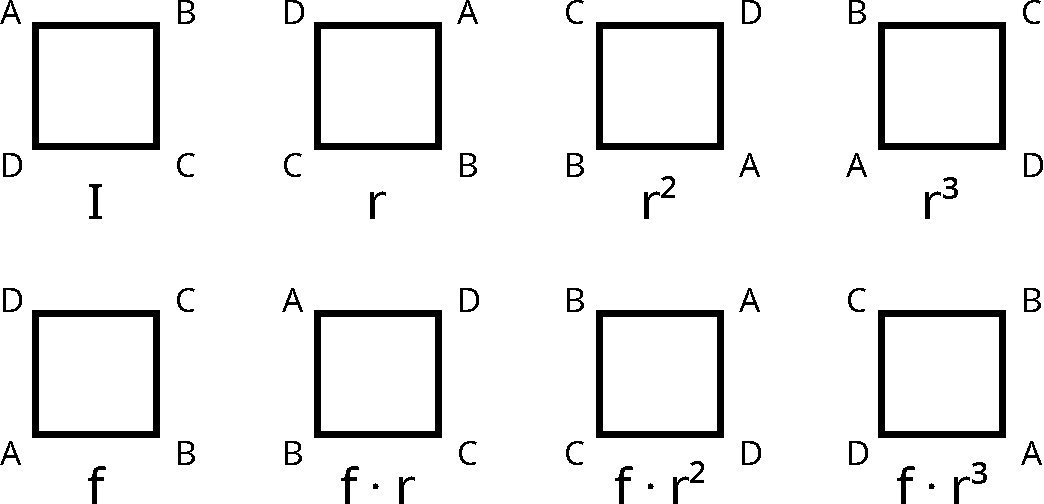
\includegraphics[width=0.8\linewidth]{figures/grupodiedral.pdf}
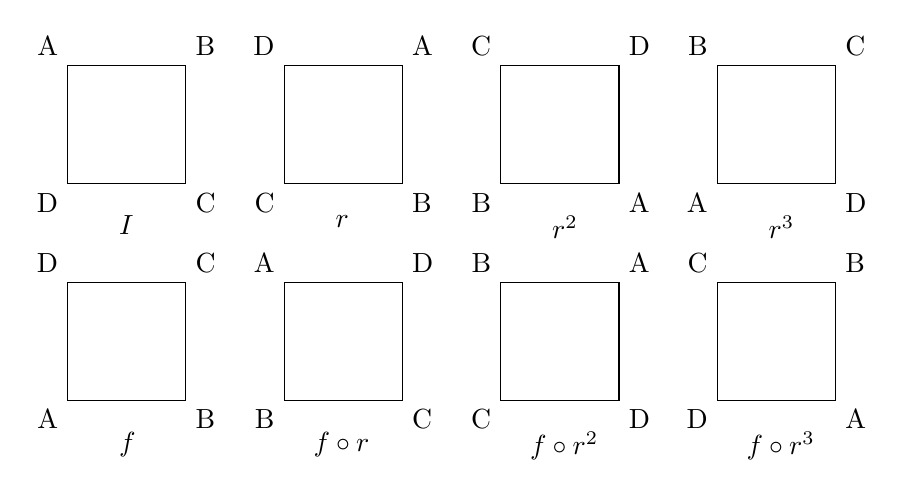
\begin{tikzpicture}

  \newcommand{\mysquare}[8]{% arguments: column, row, index
    \begin{scope}[xshift=#1*2.75cm, yshift=-#2*2.75cm] % Adjust 2.5cm for square + spacing
      \draw (0,0) node[below left] (#6) {#6}
            -- (1.5,0) node[below right] (#5) {#5}
            -- (1.5,1.5) node[above right] (#4) {#4}
            -- (0,1.5) node[above left] (#3) {#3}
            -- cycle;
      \node[below=1pt, anchor=north west, xshift=#8pt, yshift=-7pt] {#7};
    \end{scope}
  }

  % Row 1
  \mysquare{0}{0}{A}{B}{C}{D}{$I$}{15}
  \mysquare{1}{0}{D}{A}{B}{C}{$r$}{15}
  \mysquare{2}{0}{C}{D}{A}{B}{$r^2$}{15}
  \mysquare{3}{0}{B}{C}{D}{A}{$r^3$}{15}

  % Row 2
  \mysquare{0}{1}{D}{C}{B}{A}{$f$}{15}
  \mysquare{1}{1}{A}{D}{C}{B}{$f\circ r$}{7}
  \mysquare{2}{1}{B}{A}{D}{C}{$f\circ r^2$}{7}
  \mysquare{3}{1}{C}{B}{A}{D}{$f\circ r^3$}{7}

\end{tikzpicture}
\caption{As oito simetrias do quadrado, geradas pelos elementos $r$ (rotação de 90 graus no sentido horário) e $f$ (reflexão vertical), sob a operação de composição.}
\label{fig:square_symmetries}
\end{figure}

\end{example}



\begin{example}
O conjunto dos polinômios com coeficientes em $\mathbb{R}$,
denotado $\mathbb{R}[x]$, forma um grupo sob a operação de adição,
  denotado $(\mathbb{R}[x], +)$.
Dado qualquer par de polinômios, como $p(x) = x^2 + 1$ e $q(x) = 2x - 3$,
sua soma $p(x) + q(x) = x^2 + 2x - 2$ é outro polinômio em $\mathbb{R}[x]$,
satisfazendo o fecho. A adição é associativa, o elemento neutro é o polinômio zero $0$,
e o inverso de $p(x)$ é $-p(x)$, obtido ao inverter o sinal de cada coeficiente.
Este grupo é abeliano, pois $p(x) + q(x) = q(x) + p(x)$.

Note que os polinôminos não forma um grupo sob multiplicação, pois nem todo polinômio tem inverso multiplicativo.
\end{example}

\begin{example}
O conjunto das matrizes $2 \times 2$ com entradas em $\mathbb{R}$,
sob a operação de adição, também forma um grupo.
Somando duas matrizes com estas características obteremos uma outra matriz
também $2 \times 2$ com entradas em $\mathbb{R}$, ou seja, um elemento
do mesmo conjunto, demonstrando assim o fecho em relação à adição.
A adição é associativa, o elemento neutro é a matriz nula, e o inverso de uma matriz $A$ é $-A$,
obtido ao inverter o sinal de cada entrada. Este grupo é abeliano, pois a adição de matrizes é comutativa. 
\end{example}

\begin{example}
O conjunto $\mathbb{Z}/n\mathbb{Z} = \{0, 1, 2, \ldots, n-2, n-1\}$,
com a operação de adição módulo $n$, forma um grupo.
Ao tomar a soma de dois elementos em $\mathbb{Z}/6\mathbb{Z}$ obtemos
outro elemento em $\mathbb{Z}/n\mathbb{Z}$, ou seja, sejam
$a,b \in \mathbb{Z}/n\mathbb{Z}$, obtendo $c = a + b \mod n$ e
temos que $c \in \mathbb{Z}/n\mathbb{Z}$, demonstrando assim o fecho em relação
à adição. A adição é associativa, o elemento neutro é $0$, e o inverso de $a$ é $n - a$.
Este grupo é abeliano, pois a adição é comutativa. 
\end{example}



Após explorar os grupos, que possuem uma única operação binária, passamos
agora a considerar estruturas que combinam duas operações. Quando um grupo
comutativo sob a adição também é equipado com uma operação de multiplicação que
é associativa, distributiva em relação à adição e possui um elemento neutro
multiplicativo $1 \neq 0$, chamamos essa estrutura de anel.







\subsection{Anéis}

\begin{definition}[Anel]
Um anel é um conjunto $R$ equipado com duas operações binárias, tipicamente
chamadas de adição ($+$) e multiplicação ($\cdot$). Sob a adição, $R$ forma um
grupo abeliano, de modo que a adição é associativa, satisfazendo 
$(a + b) + c = a + (b + c)$ para quaisquer elementos $a$, $b$ e $c$ em $R$;
é comutativa, com $a + b = b + a$; possui um elemento neutro $0$, tal que
$a + 0 = a$ para qualquer $a$ em $R$; e cada elemento $a$ em $R$ possui um inverso
aditivo $-a$, com $a + (-a) = 0$. Sob a multiplicação, $R$ é associativo, ou seja, 
$(a \cdot b) \cdot c = a \cdot (b \cdot c)$ para quaisquer $a$, $b$ e $c$ em $R$, e
possui um elemento neutro $1$, diferente de $0$, tal que $a \cdot 1 = 1 \cdot a
= a$ para qualquer $a$ em $R$. A multiplicação é distributiva em relação à
adição, satisfazendo $a \cdot (b + c) = (a \cdot b) + (a \cdot c)$ e $(b + c)
\cdot a = (b \cdot a) + (c \cdot a)$ para quaisquer $a$, $b$ e $c$ em $R$. Um
anel é comutativo se a multiplicação for comutativa, isto é, se $a \cdot b = b
\cdot a$ para quaisquer $a$ e $b$ em $R$.
\end{definition}


Alguns autores definem anéis sem exigir a existência do elemento neutro
multiplicativo\footnote{Para esses autores, um anel que possui elemento
  neutro multiplicativo $1$ é chamado de anel com identidade, enquanto
  a definição mais geral de anel não exige tal elemento. Assim, o que chamamos
  simplesmente de ``anel'' neste livro seria, para esses autores, ``anel com
  identidade''. Optamos pela convenção moderna, que inclui a identidade por
  padrão, para alinhar com a literatura mais comum em álgebra abstrata e suas
  aplicações na teoria da codificação.}. Adotamos a definição com identidade,
pois é a mais relevante para a teoria da codificação, especialmente em anéis de
polinômios usados em códigos cíclicos e BCH.


\begin{example}
O conjunto dos inteiros $\mathbb{Z}$, com as operações usuais de adição e
multiplicação, forma um anel comutativo.
\end{example}

\begin{example}
O conjunto $\mathbb{Z}/2\mathbb{Z} = \{0, 1\}$, com adição e multiplicação
módulo 2, também forma um anel comutativo, onde $0$ é o neutro aditivo e $1$ é
o neutro multiplicativo. Ele também é conhecido como campo de Galois de ordem 2, denotado $\mathbb{F}₂ = \text{GF}(2)$.
\end{example}

\begin{example}
O conjunto de polinômios com coeficientes em $\mathbb{Z}/2\mathbb{Z}$, denotado
$\mathbb{Z}/2\mathbb{Z}[x]$, equipado com adição e multiplicação de polinômios
módulo 2, forma um anel comutativo.
\end{example}

\begin{example}
Anéis como $\mathbb{Z}/2\mathbb{Z}[x] / (x^n - 1)$
são usados para construir códigos cíclicos, como os códigos BCH, explorando
simetrias nas sequências de código.
\end{example}


Um anel comutativo com unidade, onde todo elemento não nulo possui um inverso
multiplicativo, ou seja, um anel onde é possível realizar divisão por qualquer
elemento diferente de zero, é chamado de corpo.
Por exemplo, o anel $\mathbb{Z}/2\mathbb{Z}$ é um corpo, pois o elemento $1$ é seu próprio
inverso multiplicativo $1 \cdot 1 = 1$. Em contraste, o anel $\mathbb{Z}$ não é
um corpo, pois elementos como $2$ não possuem
inverso multiplicativo em $\mathbb{Z}$: não existe inteiro $b$ tal que $2 \cdot b = 1$.
Já o anel $\mathbb{Q}$ é um corpo, pois para qualquer racional
não nulo $\frac{a}{b}$, existe um inverso $\frac{b}{a}$ tal que
$\frac{a}{b} \cdot \frac{b}{a} = 1$.






\subsection{Corpos}

\begin{definition}[Corpo]
Um corpo é um conjunto $F$ equipado com duas operações binárias, $+$
(adição) e $\cdot$ (multiplicação). Sob a adição, $F$ forma um grupo
abeliano, com um elemento neutro $0$, de modo que a adição é associativa e
comutativa, e cada elemento possui um inverso aditivo. Sob a multiplicação, o
conjunto $F \setminus \{0\}$ forma um grupo abeliano, com um elemento
neutro $1$, diferente de $0$, onde a multiplicação é associativa e
comutativa, e cada elemento não nulo $a$ em $F$ possui um inverso
multiplicativo $a^{-1}$, satisfazendo $a \cdot a^{-1} = 1$. A
multiplicação é distributiva em relação à adição, ou seja,
$a \cdot (b + c) = (a \cdot b) + (a \cdot c)$ para quaisquer $a$, $b$ e $c$ em $F$.
\end{definition}


Em termos simples, um corpo é um anel comutativo onde podemos dividir por
qualquer elemento não nulo, ou seja, todo elemento diferente de zero tem um
inverso multiplicativo. Formalmente, um corpo é um anel comutativo com unidade
no qual todo elemento não nulo possui um inverso multiplicativo, permitindo,
assim, a divisão por qualquer elemento diferente de zero, e a multiplicação
deve ser comutativa.

\begin{example}
Os conjuntos dos números racionais $\mathbb{Q}$, reais $\mathbb{R}$ e complexos $\mathbb{C}$,
com as operações usuais de adição e multiplicação, são corpos\footnote{Formalmente, um corpo
  é denotado como $(F, +, \cdot)$, onde $F$ é o conjunto e $+$ e $\cdot$ são as operações de
  adição e multiplicação, respectivamente. Assim, $\mathbb{R}$ é uma abreviação para 
  $(\mathbb{R}, +, \cdot)$, onde $+$ e $\cdot$ são as operações usuais de adição e 
  multiplicação dos números reais.}.
\end{example}

\begin{example}
O conjunto $\mathbb{Z}/2\mathbb{Z} = \{0, 1\}$, com adição e multiplicação módulo 2,
forma o corpo finito $\mathbb{F}_2$, onde $1 \cdot 1 = 1$ e $1$ é seu próprio inverso.
\end{example}

\begin{example}
Para qualquer número primo $p$, o conjunto
$\mathbb{Z}/p\mathbb{Z} = \{0, 1, \ldots, p-1\}$, com adição e multiplicação
módulo $p$, forma um corpo finito denotado $\mathbb{F}_p$. Sob a
adição, $\mathbb{Z}/p\mathbb{Z}$ é um grupo abeliano, pois a adição módulo
$p$ é associativa e comutativa, o elemento neutro é $0$, e o inverso
aditivo de $a$ é $p - a$, já que $a + (p - a) \equiv 0 \pmod{p}$.
Sob a multiplicação, o conjunto $\mathbb{Z}/p\mathbb{Z} \setminus \{0\} = \{1, 2, \ldots, p-1\}$ 
forma um grupo abeliano: a multiplicação módulo $p$ é associativa e comutativa,
o elemento neutro é $1$, e todo elemento $a \neq 0$ tem um inverso multiplicativo,
porque $p$ é primo e, portanto, $a$ e $p$ são coprimos, garantindo, pela identidade de Bézout,\footnote{
  Identidade de Bézout: para quaisquer inteiros $a$ e $b$ não ambos zero,
  existem inteiros $x$ e $y$ tais que $ax + by = \text{MDC}(a, b)$.
  Aqui, como $\text{MDC}(a, p) = 1$, temos $ax + py = 1$.% A demonstração está no \Cref{thm:bezout}.
}
a existência
de inteiros $x$ e $y$ tais que $a x + p y = 1$, ou seja, $a x \equiv 1 \pmod{p}$,
onde $x \mod p$ é o inverso de $a$. A distributividade da multiplicação
em relação à adição é válida em $\mathbb{Z}/p\mathbb{Z}$, como em qualquer
aritmética modular. Isso só é válido porque $p$ é primo; se $p$ não for
primo, como em $\mathbb{Z}/4\mathbb{Z}$, o elemento $2$ não possui
inverso multiplicativo, pois não existe $b$ tal que $2 \cdot b \equiv 1 \pmod{4}$.
\end{example}

\begin{example}
Para ilustrar as propriedades de $\mathbb{Z}/p\mathbb{Z}$ com um exemplo
concreto, considere $p = 7$, um número primo. O conjunto
$\mathbb{Z}/7\mathbb{Z} = \{0, 1, 2, 3, 4, 5, 6\}$, com adição e multiplicação
módulo 7, forma o corpo finito $\mathbb{F}_7$, também conhecido como o campo de
Galois de ordem 7, denotado GF(7). Para visualizar as operações de adição e
multiplicação, podemos usar as chamadas tabelas de Cayley, que listam os resultados
de todas as possíveis combinações de elementos sob uma operação binária.
A tabela de Cayley para a adição módulo 7 (veja a \Cref{tab:cayley_mod7}) mostra que $(\mathbb{Z}/7\mathbb{Z}, +)$
é um grupo abeliano: a operação é comutativa, o que pode ser observado pela simetria
da tabela em relação à diagonal principal (ou seja, o elemento na posição $(a, b)$
é igual ao da posição $(b, a)$, como $2 + 5 = 5 + 2 = 0$). Além disso, nenhuma
linha ou coluna contém o mesmo elemento duas vezes, garantindo que cada
elemento $b$ tem um único $a$ tal que $a + b = c$ para qualquer
$c$, o que reflete a existência de inversos aditivos. A tabela de Cayley
para a multiplicação módulo 7 (veja a \Cref{tab:cayley_mod7}) mostra que $(\mathbb{Z}/7\mathbb{Z} \setminus \{0\}, \cdot)$
também é um grupo abeliano: a multiplicação é comutativa (novamente, a tabela é
simétrica em relação à diagonal e, exceto na linha e coluna do 0 (que sempre resulta em 0),
nenhuma linha ou coluna contém o mesmo elemento não nulo duas vezes,
indicando que cada elemento $a \neq 0$ tem um único inverso
multiplicativo (por exemplo, o inverso de 3 é 5, pois $3 \cdot 5 = 1$).
Essas propriedades confirmam que $\mathbb{Z}/7\mathbb{Z}$ é um corpo.

\begin{table}[!htb]
    \centering
    \caption{Tabela de Cayley para adição e multiplicação módulo 7.}
    \label{tab:cayley_mod7}
    \begin{minipage}{.45\linewidth}
        \centering
        \begin{tabular}{c|ccccccc}
            $+$ & 0 & 1 & 2 & 3 & 4 & 5 & 6 \\
            \hline
            0 & 0 & 1 & 2 & 3 & 4 & 5 & 6 \\
            1 & 1 & 2 & 3 & 4 & 5 & 6 & 0 \\
            2 & 2 & 3 & 4 & 5 & 6 & 0 & 1 \\
            3 & 3 & 4 & 5 & 6 & 0 & 1 & 2 \\
            4 & 4 & 5 & 6 & 0 & 1 & 2 & 3 \\
            5 & 5 & 6 & 0 & 1 & 2 & 3 & 4 \\
            6 & 6 & 0 & 1 & 2 & 3 & 4 & 5 \\
        \end{tabular}
    \end{minipage}\hfill
    \begin{minipage}{.45\linewidth}
        \centering
        \begin{tabular}{c|ccccccc}
            $\cdot$ & 0 & 1 & 2 & 3 & 4 & 5 & 6 \\
            \hline
            0 & 0 & 0 & 0 & 0 & 0 & 0 & 0 \\
            1 & 0 & 1 & 2 & 3 & 4 & 5 & 6 \\
            2 & 0 & 2 & 4 & 6 & 1 & 3 & 5 \\
            3 & 0 & 3 & 6 & 2 & 5 & 1 & 4 \\
            4 & 0 & 4 & 1 & 5 & 2 & 6 & 3 \\
            5 & 0 & 5 & 3 & 1 & 6 & 4 & 2 \\
            6 & 0 & 6 & 5 & 4 & 3 & 2 & 1 \\
        \end{tabular}
    \end{minipage}
\end{table}
\end{example}

\begin{example}
Corpos finitos $\mathbb{F}_q$, também conhecidos como campos de Galois,
existem para $q = p^m$, onde $p$ é um primo e $m \geq 1$ é um
inteiro. Por exemplo, o corpo $\mathbb{F}_4$ tem como elementos $\{0, 1, \alpha, \alpha + 1\}$.
Aqui, $\mathbb{F}_4$ é construído como uma extensão de $\mathbb{F}_2$, e $\alpha$
é um elemento adicional que satisfaz a relação $\alpha^2 = \alpha + 1$,
escolhida para garantir que $\mathbb{F}_4$ tenha exatamente 4 elementos
e forme um corpo. Essa relação é derivada de um polinômio irredutível
$x^2 + x + 1$ em $\mathbb{F}_2[x]$\footnote{
  Um polinômio irredutível em $\mathbb{F}_2[x]$ é um polinômio
  que não pode ser fatorado em polinômios de grau menor, exceto por constantes. O
  polinômio $x^2 + x + 1$ é irredutível porque não tem raízes em $\mathbb{F}_2$:
  nem $x = 0$, nem $x = 1$ o satisfazem. Esse conceito
  será explorado em detalhes em capítulos futuros.},
  permitindo definir as operações em $\mathbb{F}_4$. A adição e multiplicação 
são realizadas usando essa propriedade: por exemplo, $(\alpha + 1) + \alpha = (1 + 1) = 0$ 
em $\mathbb{F}_2$, então $(\alpha + 1) + \alpha = 1$; e para a multiplicação,
$(\alpha + 1) \cdot \alpha = \alpha^2 + \alpha = (\alpha + 1) + \alpha = 1$. 
Corpos finitos como $\mathbb{F}_4$ são amplamente utilizados na teoria
da codificação: códigos Reed-Solomon usam $\mathbb{F}_q$ para codificar
mensagens como polinômios, permitindo a correção de múltiplos erros, e também
são essenciais em criptografia, como nos protocolos RSA e de curvas elípticas.
\end{example}




Uma propriedade fundamental dos corpos finitos é a existência de elementos
primitivos, que são essenciais na teoria da codificação e na criptografia. Todo
corpo finito $\mathbb{F}_q$ possui pelo menos um elemento primitivo, e o
número de elementos primitivos é dado por $\phi(q-1)$, onde $\phi$ é a
função totiente de Euler, que conta o número de inteiros positivos até $q-1$
que são coprimos com $q-1$.

\begin{definition}[Elemento Primitivo]
Um elemento $\alpha \in \mathbb{F}_q \setminus \{0\}$ de um corpo finito $\mathbb{F}_q$
é chamado de primitivo se, ao multiplicá-lo por si mesmo repetidamente ($\alpha^1, \alpha^2, \alpha^3, \ldots $),
ele gera todos os $q-1$ elementos não nulos do corpo, ou seja, o conjunto $\{ \alpha^0, \alpha^1, \alpha^2, \ldots, \alpha^{q-2} \}$,
onde $\alpha^0 = 1$, contém todos os elementos de $\mathbb{F}_q \setminus \{0\}$.
Em outras palavras, $\alpha$ é um gerador do grupo multiplicativo $(\mathbb{F}_q \setminus \{0\}, \cdot)$,
que é sempre cíclico\footnote{
  O conceito de elemento primitivo, ou gerador, não é exclusivo de corpos
  finitos. Em um grupo cíclico $(G, *)$, um elemento $g \in G$ é
  chamado de gerador se todo elemento $x \in G$ pode ser obtido aplicando
  repetidamente a operação binária $*$ a $g$ (ou seu inverso), ou seja,
  $G = \langle g \rangle$. Isso não se restringe a operações
  multiplicativas. Por exemplo, ao definir Grupos, vimos que $(\mathbb{Z}/n\mathbb{Z}, +)$
  é cíclico, e o elemento 1 é um gerador, pois $\{1, 1+1, \ldots, (n-1)+1\}$
  gera todos os elementos do grupo sob adição. 
  }.

\end{definition}

\begin{example}
Considere o corpo finito $\mathbb{F}_5 = \mathbb{Z}/5\mathbb{Z} = \{0, 1, 2, 3, 4\}$,
com $q = 5$, então $q-1 = 4$, e $\phi(4) = \phi(2^2) = 2^2 - 2^1 = 2$, indicando
que há 2 elementos primitivos. Para $\alpha = 2$, temos $2^1 = 2$, $2^2 = 4$, 
$2^3 = 8 \equiv 3 \pmod{5}$, $2^4 = 2 \cdot 3 = 6 \equiv 1 \pmod{5}$, gerando $\{1, 2, 4, 3\}$,
que contém todos os elementos de $\mathbb{F}_5 \setminus \{0\}$, então 2 é primitivo.
Para $\alpha = 3$, temos $3^1 = 3$, $3^2 = 9 \equiv 4 \pmod{5}$, $3^3 = 3 \cdot 4 = 12 \equiv 2 \pmod{5}$,
$3^4 = 3 \cdot 2 = 6 \equiv 1 \pmod{5}$, gerando $\{1, 3, 4, 2\}$, então 3 também é primitivo.
Porém, para $\alpha = 4$, temos $4^1 = 4$, $4^2 = 16 \equiv 1 \pmod{5}$, $4^3 = 4 \cdot 1 = 4$,
$4^4 = 4 \cdot 4 = 16 \equiv 1 \pmod{5}$, gerando apenas $\{1, 4\}$, que não inclui todos os
elementos não nulos, então 4 não é primitivo. Assim, 2 e 3 são os dois elementos primitivos
de $\mathbb{F}_5$, como previsto por $\phi(4) = 2$. 
\end{example}

Elementos primitivos são amplamente utilizados na teoria da codificação: em
códigos cíclicos como os códigos Reed-Solomon, eles são usados para construir
polinômios geradores, e em criptografia, como no protocolo Diffie-Hellman, eles
garantem a segurança baseada na dificuldade do logaritmo discreto em corpos
finitos.



Para explorar mais a estrutura de corpos finitos como $\mathbb{Z}/n\mathbb{Z}$,
é útil introduzir o conceito de relação de equivalência, que nos permite
organizar elementos em classes com base em uma relação que generaliza a ideia
de igualdade. Vamos, antes de explorarmos a relação de equivalência, introduzir
o conceito mais geral de relação binária.
Relações binárias são utilizadas por toda a matemática desde o início -- em comparações,
pertinência a conjuntos, divisibilidade, funções e muito mais. Embora as aplicamos
rotineiramente, podem não ter sido até então formalmente definidas. A formalização abstrai
e generaliza esses padrões familiares de associação entre elementos.

\begin{definition}[Relação Binária]
Sejam $A$ e $B$ conjuntos não vazios. Uma relação binária de $A$ para $B$ é um subconjunto
$R \subseteq A \times B$. Se $(a, b) \in R$, dizemos que $a$ está relacionado a $b$ por $R$,
e escrevemos $a R b$. Quando $A = B$, a relação é chamada de homogênea, e dizemos que $R$ é
uma relação binária em $A$.
\end{definition}

Relações binárias, especialmente as homogêneas, são usadas em muitas áreas da matemática
para modelar uma ampla variedade de conceitos. Estas incluem, entre outros: a relação
``é maior que'', ``é igual a'' e ``divide'' em aritmética; a relação ``é congruente a''
em geometria; a relação ``é adjacente a'' na teoria dos grafos; e a relação ``é ortogonal a''
em álgebra linear. Para entender as propriedades dessas relações, examinemos algumas delas
em termos de reflexividade, simetria e transitividade, que são características fundamentais
que definem tipos especiais de relações, como veremos adiante.

\begin{example}
Considere o conjunto $\mathbb{R}$ dos números reais e a relação ``igual a'' ($=$), definida por $a = b$. Esta relação é:
reflexiva, pois para qualquer $a \in \mathbb{R}$, $a=a$, ou seja, todo número é igual a si mesmo;
simétrica, pois se $a = b$, então $b = a$, pois a igualdade não depende da ordem;
e transitiva, pois se $a = b$ e $b = c$, então $a = c$, pois a igualdade é transitiva.

Agora, considere a relação ``maior que'' ($>$) em $\mathbb{R}$, definida por $a > b$. Esta relação:
não é reflexiva, pois $a > a$ é falso, pois um número não pode ser maior que ele mesmo;
não é simétrica, pois se $a > b$, então $b > a$ é falso;
é transitiva, pois se $a > b$ e $b > c$, então $a > c$.

Outro exemplo é a relação ``divide''' ($\mid$) em $\mathbb{Z}^+$, o conjunto dos inteiros positivos,
onde $a \mid b$ se existe um inteiro $k$ tal que $b = k a$. Esta relação:
é reflexiva, pois $a \mid a$, uma vez que $a = 1 \cdot a$;
não é simétrica, pois se $a \mid b$, não é garantido que $b \mid a$ (e.g., $2 \mid 4$, mas $4 \nmid 2$);
é transitiva, pois se $a \mid b$ e $b \mid c$, então $a \mid c$.
\end{example}







\begin{definition}[Relação de Equivalência]
Seja $S$ um conjunto não vazio. Uma relação binária $R$ em $S$
(isto é, um subconjunto de $S \times S$) é chamada de relação de equivalência
se satisfaz as seguintes três propriedades:
para todo $a \in S$, $(a, a) \in R$, ou seja, $a R a$ (reflexividade);
para todos $a, b \in S$, se $(a, b) \in R$, então $(b, a) \in R$, ou seja, se $a R b$, então $b R a$ (simetria);
para todos $a, b, c \in S$, se $(a, b) \in R$ e $(b, c) \in R$, então $(a, c) \in R$, ou seja, se $a R b$ e $b R c$, então $a R c$ (transitividade).
\end{definition}

Na literatura, diferentes notações são encontradas para expressar relação
de equivalência: $a \sim b$ e $a \equiv b$ são comummente utilizadas, quando
$R$ é implícito no contexto; ou $a R b$ pode ser utilizada para explicitar $R$.

Uma relação de equivalência $R$ em um conjunto $S$ induz uma partição de $S$,
ou seja, $S$ pode ser expresso como a união de subconjuntos não vazios e disjuntos
(isto é, subconjuntos que não têm elementos em comum), chamados de classes de equivalência.

\begin{definition}[Classe de Equivalência]
Dada uma relação de equivalência $R$ em um conjunto $S$, a classe de equivalência
de um elemento $a \in S$, denotada $[a]$, é o conjunto de todos os elementos de $S$
que estão relacionados a $a$ sob $R$, ou seja, $[a] = \{ x \in S \mid x R a \}$.
O conjunto das classes de equivalência forma uma partição de $S$, pois $S$ é a
união disjunta de todas as classes $[a]$ para $a \in S$, e duas classes $[a]$ e
$[b]$ são iguais ou disjuntas (se $[a] \cap [b] \neq \emptyset$, então $[a] = [b]$).
\end{definition}

Um exemplo importante de relação de equivalência surge na aritmética modular,
que já encontramos em corpos finitos como $\mathbb{Z}/n\mathbb{Z}$.

\begin{example}
Sejam $\mathbb{Z}$ o conjunto dos inteiros e $n \geq 1$ um inteiro fixo.
Definimos a relação de congruência módulo $n$ dizendo que $a \equiv b \pmod{n}$ se $n$
divide $a - b$, ou seja, $a - b = k n$ para algum inteiro $k$.
Vamos verificar que esta é uma relação de equivalência em $\mathbb{Z}$:
para qualquer $a \in \mathbb{Z}$, $a - a = 0 = 0 \cdot n$, então $a \equiv a \pmod{n}$ (reflexividade);
se $a \equiv b \pmod{n}$, então $a - b = k n$, e $b - a = -k n$, onde $-k$ é um inteiro, então $b \equiv a \pmod{n}$ (simetria);
se $a \equiv b \pmod{n}$ e $b \equiv c \pmod{n}$, então $a - b = k n$ e $b - c = m n$, e somando, $a - c = (a - b) + (b - c) = k n + m n = (k + m) n$ (transitividade).

As classes de equivalência desta relação são os conjuntos $[a] = \{ x \in \mathbb{Z} \mid x \equiv a \pmod{n} \}$,
que correspondem aos restos possíveis ao dividir por $n$: $[0], [1], \ldots, [n-1]$.
Por exemplo, para $n = 5$, a classe $[2] = \{ \ldots, -8, -3, 2, 7, 12, \ldots \}$,
e o conjunto das classes $\{ [0], [1], [2], [3], [4] \}$ forma uma partição de $\mathbb{Z}$.
Este conjunto de classes de equivalência é exatamente o corpo finito $\mathbb{Z}/5\mathbb{Z}$
(ou $\mathbb{F}_5$) quando $n = 5$ é primo, como vimos anteriormente.
\end{example}










Agora que entendemos a relação de congruência e como ela particiona
$\mathbb{Z}$ em classes de equivalência, podemos explorar um conceito
relacionado que surge naturalmente ao estudar grupos e seus subgrupos: as
coclasses. Este conceito nos ajuda a compreender a estrutura de grupos como
$\mathbb{Z}/n\mathbb{Z}$ e será útil em aplicações futuras na teoria da
codificação.

\begin{definition}[Coclasse]
Seja $G$ um grupo e $H$ um subgrupo de $G$. Para qualquer elemento $x \in G$,
definimos a coclasse à esquerda de $H$ em $G$ com
representante $x$, denotada $xH$, como o conjunto $xH = \{ xh \mid h \in H \}$,
onde $x$ é fixo e $h$ varia sobre todos os elementos
de $H$. Similarmente, definimos a coclasse à direita de $H$ em
$G$ com representante $x$, denotada $Hx$, como o conjunto
$Hx = \{ hx \mid h \in H \}$. Como $H \subseteq G$ e $x \in G$, e $G$
é fechado sob sua operação, todos os elementos $xh$ (ou $hx$)
pertencem a $G$, de modo que cada coclasse é um subconjunto de $G$,
embora os elementos de $xH$ ou $Hx$ não precisem pertencer a $H$.
\end{definition}

As coclasses de um subgrupo $H$ em $G$ têm uma propriedade importante:
elas formam uma partição de $G$. Isso significa que $G$ é a união
disjunta das coclasses à esquerda $aH$ (ou à direita $Ha$) para todos
$a \in G$. O conjunto das coclasses à esquerda é denotado por
$G/H = \{ aH \mid a \in G \}$. Além disso, as coclasses satisfazem a seguinte
propriedade: se duas coclasses à esquerda $aH$ e $bH$ possuem algum
elemento em comum, então elas são iguais. Para ver isso, suponha que
$c \in aH \cap bH$. Então, $c = ah_1$ para algum $h_1 \in H$ e $c = bh_2$
para algum $h_2 \in H$. Assim, $ah_1 = bh_2$, e multiplicando ambos
os lados à direita por $h_1^{-1}$, temos $a = b(h_2 h_1^{-1})$. Como
$H$ é um subgrupo, $h_2 h_1^{-1} \in H$, então $a = bk$ para algum
$k \in H$, e $aH = (bk)H = b(kH) = bH$, já que $kH = H$\footnote{
  A igualdade $kH = H$ ocorre porque $H$ é um subgrupo de $G$.
  Primeiro, $H$ é fechado sob a operação: se $h_1, h_2 \in H$,
  então $h_1 h_2 \in H$. Assim, para qualquer $h \in H$, $kh \in H$
  (já que $k \in H$), e $kH \subseteq H$. Segundo, $H$ contém
  os inversos: para cada $h \in H$, existe $h^{-1} \in H$ tal que
  $h h^{-1} = e$, onde $e$ é o elemento neutro de $G$. Como $k \in H$,
  existe $k^{-1} \in H$, e para qualquer $h' \in H$, podemos escrever
  $h' = k (k^{-1} h')$, onde $k^{-1} h' \in H$ (pois $H$ é fechado).
  Assim, $h' \in kH$, e $H \subseteq kH$. Portanto, $kH = H$.}.
Uma demonstração análoga vale para coclasses à direita.

\begin{example}
Considere o grupo $(\mathbb{Z}/6\mathbb{Z}, +) = \{0, 1, 2, 3, 4, 5\}$, com
adição módulo 6, que já encontramos na subseção ``Grupos''. Vamos escolher o
subgrupo $H = \{0, 3\}$, que é um subgrupo porque $0 + 0 = 0$, $0 + 3 = 3$,
$3 + 3 = 6 \equiv 0 \pmod{6}$, e $H$ é fechado sob adição e
contém os inversos (o inverso de 0 é 0, e o inverso de 3 é 3, pois $3 + 3 = 0$).
As coclasses à esquerda de $H$ em $\mathbb{Z}/6\mathbb{Z}$ são:
\begin{itemize}
    \item $0 + H = \{0+0, 0+3\} = \{0, 3\}$,
    \item $1 + H = \{1+0, 1+3\} = \{1, 4\}$,
    \item $2 + H = \{2+0, 2+3\} = \{2, 5\}$,
    \item $3 + H = \{3+0, 3+3\} = \{3, 0\} = 0 + H$,
    \item $4 + H = \{4+0, 4+3\} = \{4, 1\} = 1 + H$,
    \item $5 + H = \{5+0, 5+3\} = \{5, 2\} = 2 + H$.
\end{itemize}
Observamos que há apenas três coclasses distintas: $\{0, 3\}$, $\{1, 4\}$,
e $\{2, 5\}$, que são disjuntas e cuja união é $\mathbb{Z}/6\mathbb{Z}$,
confirmando que formam uma partição. Note que $3 + H = 0 + H$, pois 
$3 \in H$, e de fato $0 + H$ e $3 + H$ têm
elementos em comum (0 e 3), o que implica que são a mesma coclasse, como
previsto pela propriedade mencionada. Como o grupo é abeliano, as coclasses à
esquerda e à direita coincidem (e.g., $H + 1 = 1 + H$). As coclasses são
fundamentais na teoria dos grupos e têm aplicações na teoria da codificação,
como na construção de códigos de grupo, onde a estrutura de partição ajuda a
definir palavras-código.
\end{example}


\begin{remark}
Uma propriedade importante das coclasses é que existe uma única coclasse que
contém o elemento identidade $e$ de $G$, e ela é o próprio subgrupo
$H$. Para coclasses à esquerda, se $xH$ contém $e$, então $e = xh$
para algum $h \in H$, o que implica $x = e h^{-1}$. Como $h^{-1} \in H$,
temos $x \in H$, e $xH = H$, já que $x \in H$.
Assim, a única coclasse à esquerda contendo $e$ é $eH = H$. O mesmo
vale para coclasses à direita: $He = H$. 
\end{remark}

Esta propriedade é fundamental
na teoria da codificação, pois em códigos de grupo, como os códigos lineares
sobre corpos finitos, o subgrupo $H$ frequentemente representa o
subespaço das palavras-código nulas, e as coclasses correspondem a traduções
desse subespaço, organizando o espaço de códigos em classes disjuntas.


\begin{remark}
Já observamos que as coclasses de um subgrupo $H$ em um grupo $G$
formam uma partição de $G$. Para enfatizar, isso significa que $G$ é
a união disjunta das coclasses à esquerda $aH$ (ou à direita $Ha$)
para $a \in G$. Em outras palavras, cada elemento de $G$ pertence a
exatamente uma coclasse: se um elemento $g \in G$ está na coclasse $aH$,
ele não pode estar em outra coclasse $bH$ com $bH \neq aH$, pois,
como demonstramos anteriormente, se $g \in aH \cap bH$, então $aH = bH$.
Assim, as coclasses são disjuntas (ou seja, $aH \cap bH = \emptyset$
se $aH \neq bH$) e sua união é todo o grupo $G$, caracterizando uma
partição.
\end{remark}


Uma consequência importante da estrutura de coclasses é que todas elas possuem
o mesmo número de elementos, uma propriedade que desempenha um papel
fundamental na teoria dos grupos e em aplicações como a teoria da codificação.

\begin{theorem}
Seja $G$ um grupo e $H$ um subgrupo de $G$. Então, toda coclasse à esquerda
$aH$ (ou à direita $Ha$) de $H$ em $G$ tem o mesmo número de elementos que
$H$, ou seja, $|aH| = |H|$ para todo $a \in G$.
\end{theorem}

\begin{proof}
Vamos mostrar que $|aH| = |H|$ para qualquer $a \in G$. Considere a coclasse à
esquerda $aH = \{ ah \mid h \in H \}$. Para provar que $|aH| = |H|$,
definimos uma função $f: H \to aH$ dada por $f(h) = ah$. Vamos mostrar que
$f$ é uma bijeção:
\begin{itemize}
\item \emph{Injetividade}: Se $f(h_1) = f(h_2)$, então $ah_1 = ah_2$.
    Multiplicando ambos os lados à
    esquerda por $a^{-1}$ (que existe, pois $G$ é um grupo), temos
    $a^{-1}(ah_1) = a^{-1}(ah_2)$, ou seja, $(a^{-1}a)h_1 = (a^{-1}a)h_2$. Como
    $a^{-1}a = e$, isso implica $h_1 = h_2$. Portanto, $f$ é injetiva.
    \item \emph{Sobrejetividade}: Para qualquer elemento $y \in aH$, existe $h
      \in H$ tal que $y = ah$. Assim, $y = f(h)$, e $f$ é sobrejetiva.
    \item \emph{Bijeção}: Como $f$ é injetiva e sobrejetiva, ela é uma bijeção
      de $H$ para $aH$, o que implica que $|H| = |aH|$.
\end{itemize}
Portanto, $|aH| = |H|$ para todo $a \in G$. Uma demonstração análoga mostra que
$|Ha| = |H|$ para coclasses à direita, definindo $f: H \to Ha$ por $f(h) = ha$.
Assim, todas as coclasses de $H$ em $G$ têm o mesmo número de elementos que $H$.
\end{proof}

\begin{remark}
Esta propriedade é essencial na teoria da codificação, especialmente em códigos
de grupo e códigos lineares sobre corpos finitos. Como $G$ é particionado em
coclasses disjuntas, e cada coclasse tem $|H|$ elementos, o número de
coclasses distintas é $|G|/|H|$, chamado de \emph{índice} de $H$ em $G$,
denotado $[G:H]$. Em códigos de grupo, isso determina o número de classes de
palavras-código, e o tamanho uniforme das coclasses garante uma estrutura
simétrica que facilita a construção e análise de códigos.
\end{remark}





Um resultado clássico da teoria dos grupos, que decorre diretamente das
propriedades das coclasses, é o Teorema de Lagrange, que estabelece uma relação
entre a ordem de um grupo e a ordem de seus subgrupos.

\begin{theorem}[Teorema de Lagrange]
Seja $G$ um grupo finito e $H$ um subgrupo de $G$. Então, a ordem de $H$,
denotada $|H|$, divide a ordem de $G$, denotada $|G|$. Em outras palavras,
$|G|/|H|$ é um inteiro, e esse inteiro é igual ao número de coclasses
distintas de $H$ em $G$, ou seja, $|G|/|H| = [G:H]$.
\end{theorem}

\begin{proof}
Já mostramos que $G$ é particionado em coclasses disjuntas $aH$, onde $a$ varia
sobre um conjunto de representantes distintos, e que cada coclasse $aH$ tem
$|H|$ elementos. Como as coclasses são disjuntas e sua união é $G$, o número
total de elementos de $G$ é o número de coclasses distintas multiplicado pelo
número de elementos em cada coclasse. O número de coclasses distintas é
um inteiro $n = [G:H]$, o índice de $H$ em $G$, então:
\begin{equation}
|G| = [G:H] \cdot |H| ,
\end{equation}
e assim obtemos
\begin{equation}
[G:H] = \frac{|G|}{|H|}
\end{equation}
Como $[G:H]$ é o número de coclasses distintas (um inteiro), $|G|/|H|$ é um
inteiro, ou seja, $|H|$ divide $|G|$. A demonstração para coclasses à direita
é análoga.
\end{proof}

\begin{remark}
Uma consequência interessante do Teorema de Lagrange ocorre quando $G$ é um
grupo finito de ordem $p$, onde $p$ é um número primo. Nesse caso, a ordem de
qualquer subgrupo $H$ de $G$ deve dividir $p$. Como $p$ é primo, os divisores
de $p$ são apenas 1 e $p$. Assim:
se $|H| = 1$, então $H = \{e\}$, o subgrupo trivial, e as coclasses
$aH = \{a\}$ têm cardinalidade 1, havendo $p$ coclasses (uma para cada elemento de $G$);
se $|H| = p$, então $H = G$, e a única coclasse é $aH = G$, que tem cardinalidade $p$.
\end{remark}

Portanto, as coclasses de qualquer subgrupo de $G$ só podem ter cardinalidade 1
ou $p$. Essa propriedade é particularmente útil na teoria da codificação e na
criptografia. Por exemplo, em corpos finitos como $\mathbb{F}_p$, o grupo
multiplicativo $(\mathbb{F}_p \setminus \{0\}, \cdot)$ tem ordem $p-1$, e
seus subgrupos (que definem subestruturas multiplicativas) têm ordens que
dividem $p-1$.

Na construção de códigos cíclicos, como os códigos
Reed-Solomon, ou em esquemas criptográficos baseados em corpos finitos (como
o protocolo Diffie-Hellman), a estrutura de subgrupos de ordem prima facilita
a escolha de elementos primitivos e a organização de palavras-código em
classes de tamanho uniforme.

